% ============================================================
%  Introducción a CMSIS-RTOS v2  —  M. Ruiz  UPM
%  Versión revisada 2025-06
% ============================================================

% ============================================================
\section{Introducción}
% ============================================================

\begin{frame}{Desarrollo de aplicaciones con Microprocesadores}
    \begin{itemize}
        \item \textbf{Aplicaciones sencillas}: implementables con un bucle
              \texttt{while}, algunos timers y algunas interrupciones.
        \item Al crecer la complejidad:
              \begin{itemize}
                  \item El número de temporizaciones supera los timers
                        hardware disponibles.
                  \item La lógica de control se vuelve difícil de gestionar
                        y depurar.
              \end{itemize}
        \item \textbf{Solución}: Sistemas Operativos de Tiempo Real (RTOS)
              \emph{ligeros}, diseñados para microprocesadores.

              $\Rightarrow$ Desarrollo más sencillo, seguro y eficiente;
              mantenimiento simplificado.
    \end{itemize}
\end{frame}

% -- Diagrama ecosistema CMSIS --------------------------------
\begin{frame}{CMSIS-RTOS}
    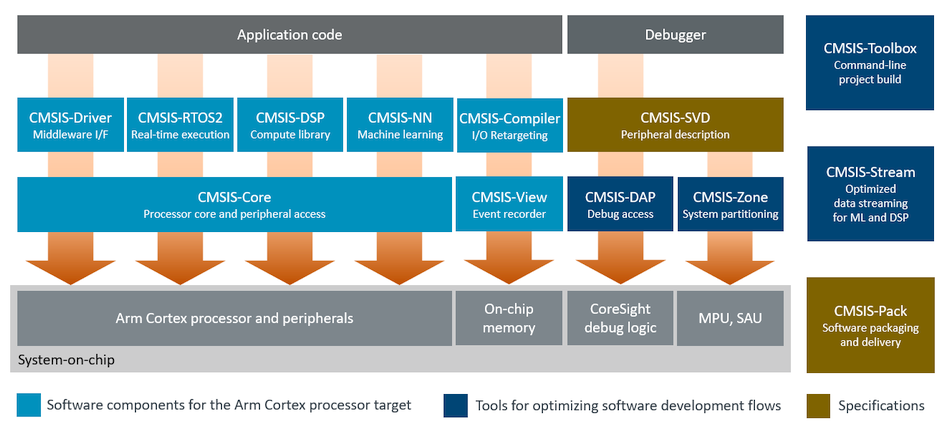
\includegraphics[scale=0.35]{cmsis_components.png}
    \begin{block}{}
        \centering
        En esta asignatura usamos \textbf{CMSIS-RTOS2} y \textbf{CMSIS-Driver}
    \end{block}
\end{frame}

% -- Qué es CMSIS-RTOS ----------------------------------------
\begin{frame}{CMSIS-RTOS}
    \begin{itemize}
        \item API C/C++ para sistemas operativos en tiempo real sobre               procesadores \textbf{Cortex-M}.
        \item Versión en uso: \textbf{CMSIS-RTOS2}. Puede ejecutarse sobre
              distintos kernels: RTX5 (Keil MDK), FreeRTOS, Zephyr, embOS,
              Azure RTOS (ThreadX), Micrium.
        \item Versión más reciente: 2.3.0 (CMSIS~v6).
              \href{https://arm-software.github.io/CMSIS_6/latest/RTOS2/index.html}
              {[Documentación 2.3.0]}
    \end{itemize}
\end{frame}

% ============================================================
\section[Características]{CMSIS-RTOS: Características}
% ============================================================

\begin{frame}{CMSIS-RTOS: Características}
    \begin{itemize}
        \item \textbf{Aplicaciones multihilo}: varios \emph{threads} se
              ejecutan de forma concurrente compartiendo la CPU.
        \item Proporciona mecanismos de \textbf{comunicación y
              sincronización}: flags, semáforos, mutexes, colas\ldots
        \item \textbf{¿Qué es un Thread?}:
            \begin{itemize}
                \item Porción de código que realiza una función concreta.
                \item Típicamente: función con bucle infinito y sin retorno.
                \item 5 estados: \texttt{Running}, \texttt{Ready},
                      \texttt{Blocked/Waiting}, \texttt{Terminated},
                      \texttt{Inactive}.
            \end{itemize}
        \item ¿Quién organiza la ejecución? \textbf{El Scheduler}: planifica y reparte el tiempo de CPU              entre threads mediante el timer \texttt{SysTick} (1\,ms por defecto).
        \item \textbf{Timeslice}: porción de tiempo asignada a cada thread
              (por defecto 5~ticks = 5\,ms).
    \end{itemize}
\end{frame}

\begin{frame}{CMSIS-RTOS: Planificador. Modos de operación}
    \begin{itemize}
        \item \textbf{Pre-emptive}: un thread de mayor prioridad desaloja
              al que está en ejecución.
        \item \textbf{Round-Robin}: todos los threads con la misma
              prioridad; se turnan cada \emph{timeslice}. Es el que vamos a utilizar en SBM.
        \item \textbf{Round-Robin Pre-emptive} \emph{(por defecto en RTX5)}:
            \begin{itemize}
                \item Los hilos pueden tener distinta prioridad.
                \item Los de igual prioridad se turnan con Round-Robin mientras no haya alguno de mayor prioridad en \texttt{READY}.
                \item \alert{Cuidado}: un thread de alta prioridad que nunca se bloquea impide la ejecución del resto.
            \end{itemize}
        \item \textbf{Cooperative Multitasking}: todos con igual prioridad; cada thread cede la CPU con \texttt{osThreadYield} o al
              bloquearse.
    \end{itemize}
\end{frame}

\begin{frame}{CMSIS-RTOS: Estados de un Thread}
    \begin{itemize}
        \item El \textbf{scheduler} gestiona las transiciones entre estados.
        \item Estados:
            \begin{itemize}
                \item \textbf{RUNNING}: thread en ejecución                  (uno solo en monocore).
                \item \textbf{READY}: preparado; espera que el scheduler                      le asigne la CPU.
                \item \textbf{BLOCKED/WAITING}: esperando un evento          (flag, semáforo, cola, delay\ldots).
                \item \textbf{TERMINATED}: ha finalizado pero el Thread Control Block (TCB) aún no ha sido liberado.
                \item \textbf{INACTIVE}: no creado, o eliminado con
                      \texttt{osThreadDelete}. No consume recursos.
            \end{itemize}
    \end{itemize}
    \vspace{4pt}
    {\footnotesize \textbf{TERMINATED} e \textbf{INACTIVE} son estados
     distintos: un thread terminado conserva su TCB hasta que se llama
     explícitamente a \texttt{osThreadDelete}.}
\end{frame}

% -- Máquina de estados (INACTIVE y TERMINATED separados) ----
\begin{frame}{Máquina de estados de un Thread}
    \begin{center}
        \resizebox{0.85\textwidth}{!}{
        \begin{tikzpicture}[shorten >=1pt, node distance=8cm,
                            on grid, auto,
                            font=\fontsize{18}{22}\selectfont,
                            line width=3pt]
            \node[state, minimum size=3cm, fill=orange]  (ready)
                {ready};
            \node[state, minimum size=3cm, fill=green]   (running)
                [right=of ready]   {running};
            \node[state, minimum size=3cm, fill=red]     (blocked)
                [right=of running] {blocked};
            \node[state, minimum size=3cm, fill=gray!60] (term)
                [below=6cm of running] {terminated};
            \node[state, minimum size=3cm, fill=gray!25] (inactive)
                [below=6cm of ready]   {inactive};

            \path[->]
                (inactive) edge node {create}           (ready)
                (ready)    edge [bend right=20] node {\textcolor{blue}{schedule}} (running)
                (running)  edge [bend right=15] node {preempt} (ready)
                (running)  edge [bend left=20]
                               node {\textcolor{blue}{wait}} (blocked)
                %(blocked)  edge [bend left=20]
                %               node {events occur}      (running)
                (blocked)  edge [bend right=35]
                               node {events occur}      (ready)
                (running)  edge node {terminate}        (term)
                (blocked)  edge node {terminate}        (term)
                (term)     edge node {osThreadDelete}   (inactive);
        \end{tikzpicture}
        }
    \end{center}
    {\footnotesize
     \textbf{INACTIVE} y \textbf{TERMINATED} son estados distintos.
     TERMINATED libera la CPU pero conserva el TCB.
     INACTIVE no consume ningún recurso del SO.}
\end{frame}

% ============================================================
\section[Código]{Código básico}
% ============================================================

% -- Crear un thread: estructura mínima ----------------------
\begin{frame}[fragile]{Ejemplo de Thread básico}
    \begin{minted}[fontsize=\scriptsize, bgcolor=blue!5]{c}
#include "cmsis_os2.h"

static osThreadId_t tid_myThread;  // static: visible solo en este módulo

void MyThread(void *argument) {
    // código de inicialización (se ejecuta una sola vez)
    while (1) {
        // código periódico
        osDelay(500);   // bloquea 500 ms y libera la CPU
    }
}

int Init_MyThread(void) {
    // osThreadAttr_t permite fijar nombre, pila y prioridad
    const osThreadAttr_t attr = { .name = "MyThread" };
    tid_myThread = osThreadNew(MyThread, NULL, &attr);
    if (tid_myThread == NULL) { return -1; }
    return 0;
}
    \end{minted}
    \begin{itemize}
        \item Usa \texttt{osThreadAttr\_t} para asignar nombre al thread:
              aparece en la Watch Window RTX y facilita la depuración.
        \item Llama siempre a \texttt{osDelay} (u otra función bloqueante)
              dentro del bucle: libera la CPU para otros threads.
    \end{itemize}
\end{frame}

% -- Estructura de ficheros -----------------------------------
\begin{frame}[fragile]{Implementación de aplicaciones con Threads}
    \begin{columns}
        \begin{column}{0.50\textwidth}
            \begin{minted}[fontsize=\scriptsize, bgcolor=blue!5]{c}
// ThDisplay.h
#ifndef __THDISPLAY_H
#define __THDISPLAY_H
#include "stm32f4xx_hal.h"
#define S_PINTA  0x0001U
int Init_ThDisplay(void);
#endif
            \end{minted}
            \begin{minted}[fontsize=\scriptsize, bgcolor=blue!5]{c}
// ThDisplay.c
#include "cmsis_os2.h"
#include "ThDisplay.h"

// static: no visible fuera de este fichero
static osThreadId_t tid_ThDisplay;

static void ThDisplay(void *arg) {
    int ciclo = 0;
    Init_display();
    while (1) {
        /* ... */
        ciclo++;
        osDelay(100);
    }
}

int Init_ThDisplay(void) {
    tid_ThDisplay = osThreadNew(
        ThDisplay, NULL, NULL);
    if (tid_ThDisplay == NULL)
        return -1;
    return 0;
}
            \end{minted}
        \end{column}
        \begin{column}{0.50\textwidth}
            \begin{minted}[fontsize=\scriptsize, bgcolor=blue!5]{c}
// main.c
#include "ThDisplay.h"

int main(void) {
    HAL_Init();
    SystemClock_Config();
    SystemCoreClockUpdate();
#ifdef RTE_CMSIS_RTOS2
    osKernelInitialize();      // correcto
    Init_ThDisplay();
    osKernelStart();
    // no retorna
#endif
    while (1);
}
            \end{minted}
            \begin{block}{Buena práctica}
                Cada periférico $\rightarrow$ un módulo
                \texttt{ThX.c/ThX.h} con su thread
                y sus objetos de sincronización.
            \end{block}
        \end{column}
    \end{columns}
\end{frame}

% -- Delays --------------------------------------------------
\begin{frame}[fragile]{Retardos y temporización}
    \begin{itemize}
        \item Basados en el \textbf{SysTick} (1~tick = 1\,ms por defecto).
        \item \alert{No se pueden usar desde una ISR.}
    \end{itemize}
    \begin{minted}[fontsize=\scriptsize, bgcolor=blue!5]{c}
// Retardo relativo — puede acumular deriva en bucles
osDelay(1000);                         // espera ~1 s

// Retardo absoluto — referencia fija, sin deriva acumulada
uint32_t tick = osKernelGetTickCount();
for (;;) {
    tick += 1000U;
    osDelayUntil(tick);                // despierta en exactamente 'tick'
    /* tarea periódica cada 1 s */
}
    \end{minted}
    \begin{columns}
        \begin{column}{0.48\textwidth}
            \begin{exampleblock}{\texttt{osDelay} — relativo}
                Cada llamada puede llegar hasta
                1~tick tarde. El error se acumula
                en bucles largos.
            \end{exampleblock}
        \end{column}
        \begin{column}{0.48\textwidth}
            \begin{exampleblock}{\texttt{osDelayUntil} — absoluto}
                La referencia es absoluta: el error
                no se acumula. Ideal para tareas
                con periodo estricto.
            \end{exampleblock}
        \end{column}
    \end{columns}
\end{frame}

% ============================================================
\section{Sincronización}
% ============================================================

% -- Motivación sincronización --------------------------------
\begin{frame}{CMSIS-RTOS: Sincronización — el problema}
    \begin{columns}
        \begin{column}{0.6\textwidth}
            \begin{itemize}
                \item Varios threads se ejecutan \textbf{concurrentemente} y pueden acceder al mismo recurso hardware o software.
                \item Sin control: los accesos se \textbf{entrelazan} y el recurso queda en estado inconsistente.
                \item El SO proporciona mecanismos para garantizar el acceso \textbf{secuencial}.
            \end{itemize}
            \vspace{6pt}
            \begin{tabular}{ll}
                \hline
                \textbf{Mecanismo} & \textbf{Uso principal} \\
                \hline
                Mutex        & Exclusión mutua \\
                Semáforo     & Señalización/conteo \\
                Thread Flags & Señal a un thread \\
                Event Flags  & Señal a N threads \\
                Cola         & Paso de datos \\
                \hline
            \end{tabular}
        \end{column}
        \begin{column}{0.40\textwidth}
            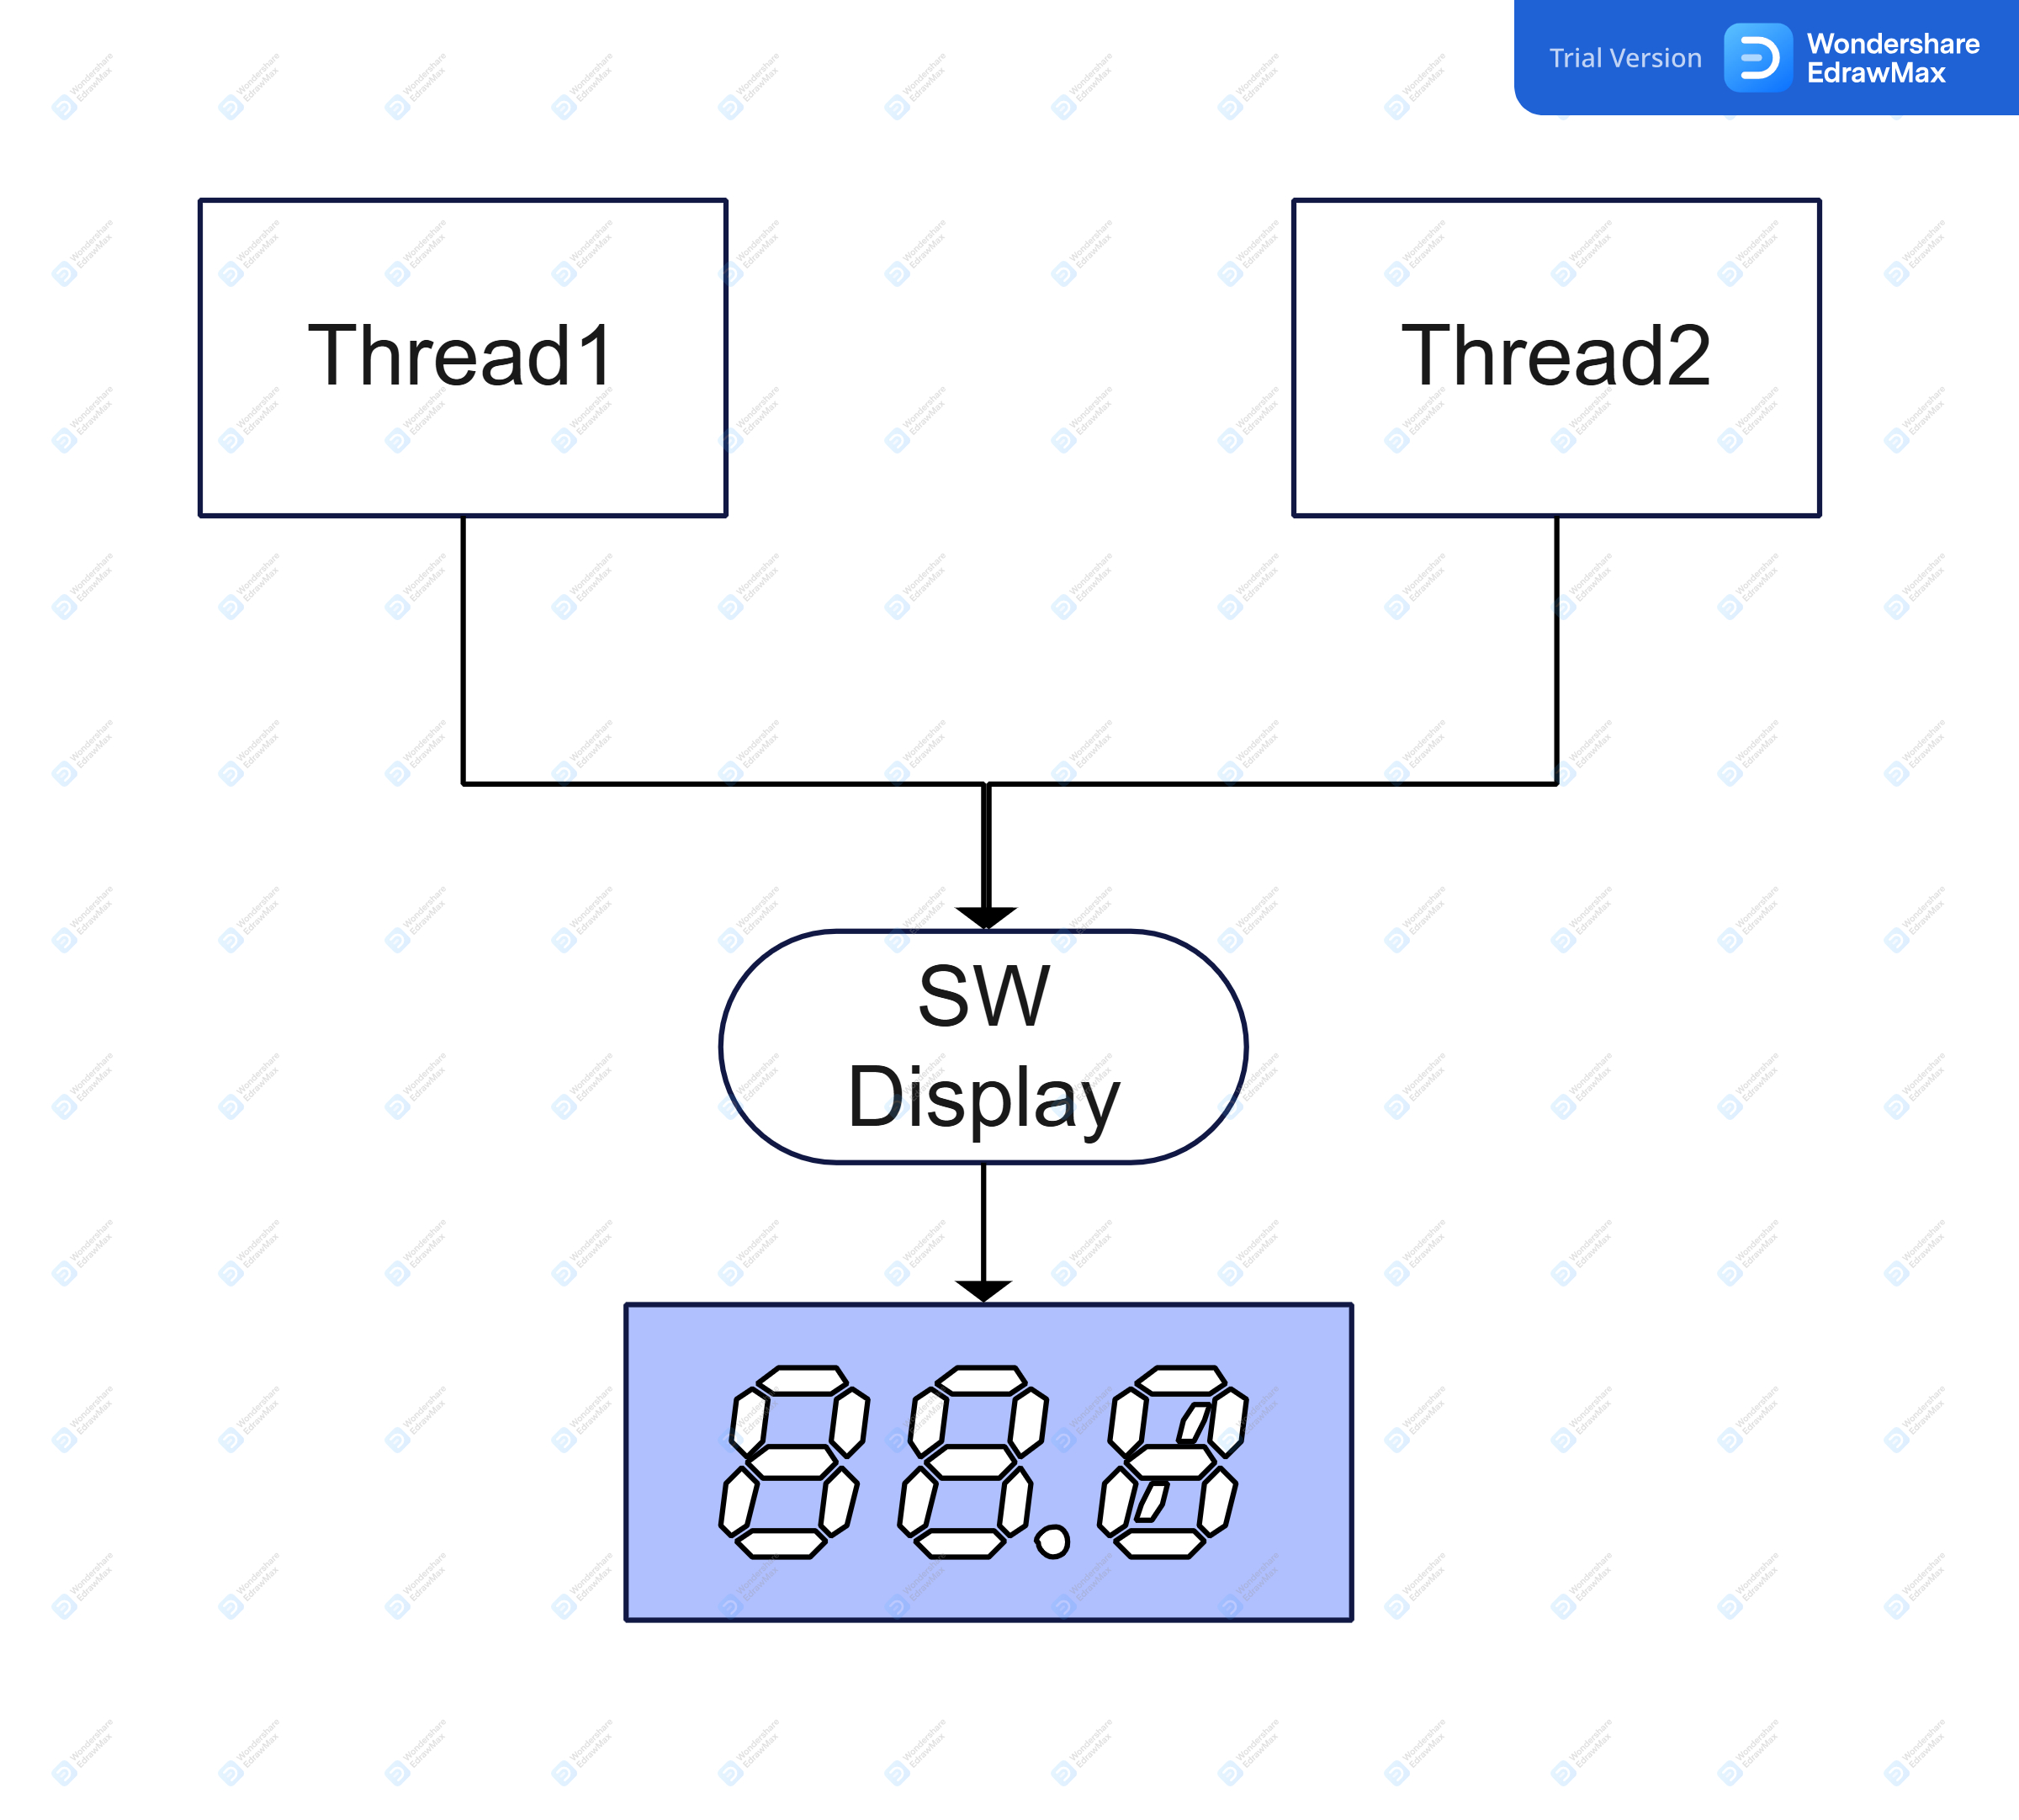
\includegraphics[scale=0.05]{threads.jpg}
        \end{column}
    \end{columns}
     \begin{exampleblock}{Importante}
        En SBM no vamos a usar Event Flags, ni Mutex ni los semáforos porque vamos a simplificar la sincronización usando Colas y Thread Flags fundamentalmente
     \end{exampleblock}
\end{frame}

% -- Solución con cola ----------------------------------------
\begin{frame}{CMSIS-RTOS: Sincronización. Una posible solución}
    \begin{columns}
        \begin{column}{0.50\textwidth}
            \begin{itemize}
                \item Se añade una \textbf{cola} gestionada por el SO.
                \item Un thread dedicado lee los mensajes de la cola y
                      los envía al display.
                \item Cada thread que quiere escribir en el LCD deposita
                      su mensaje en la cola.
                \item La cola garantiza el acceso secuencial sin que los
                      threads productores se bloqueen entre sí.
            \end{itemize}
        \end{column}
        \begin{column}{0.50\textwidth}
            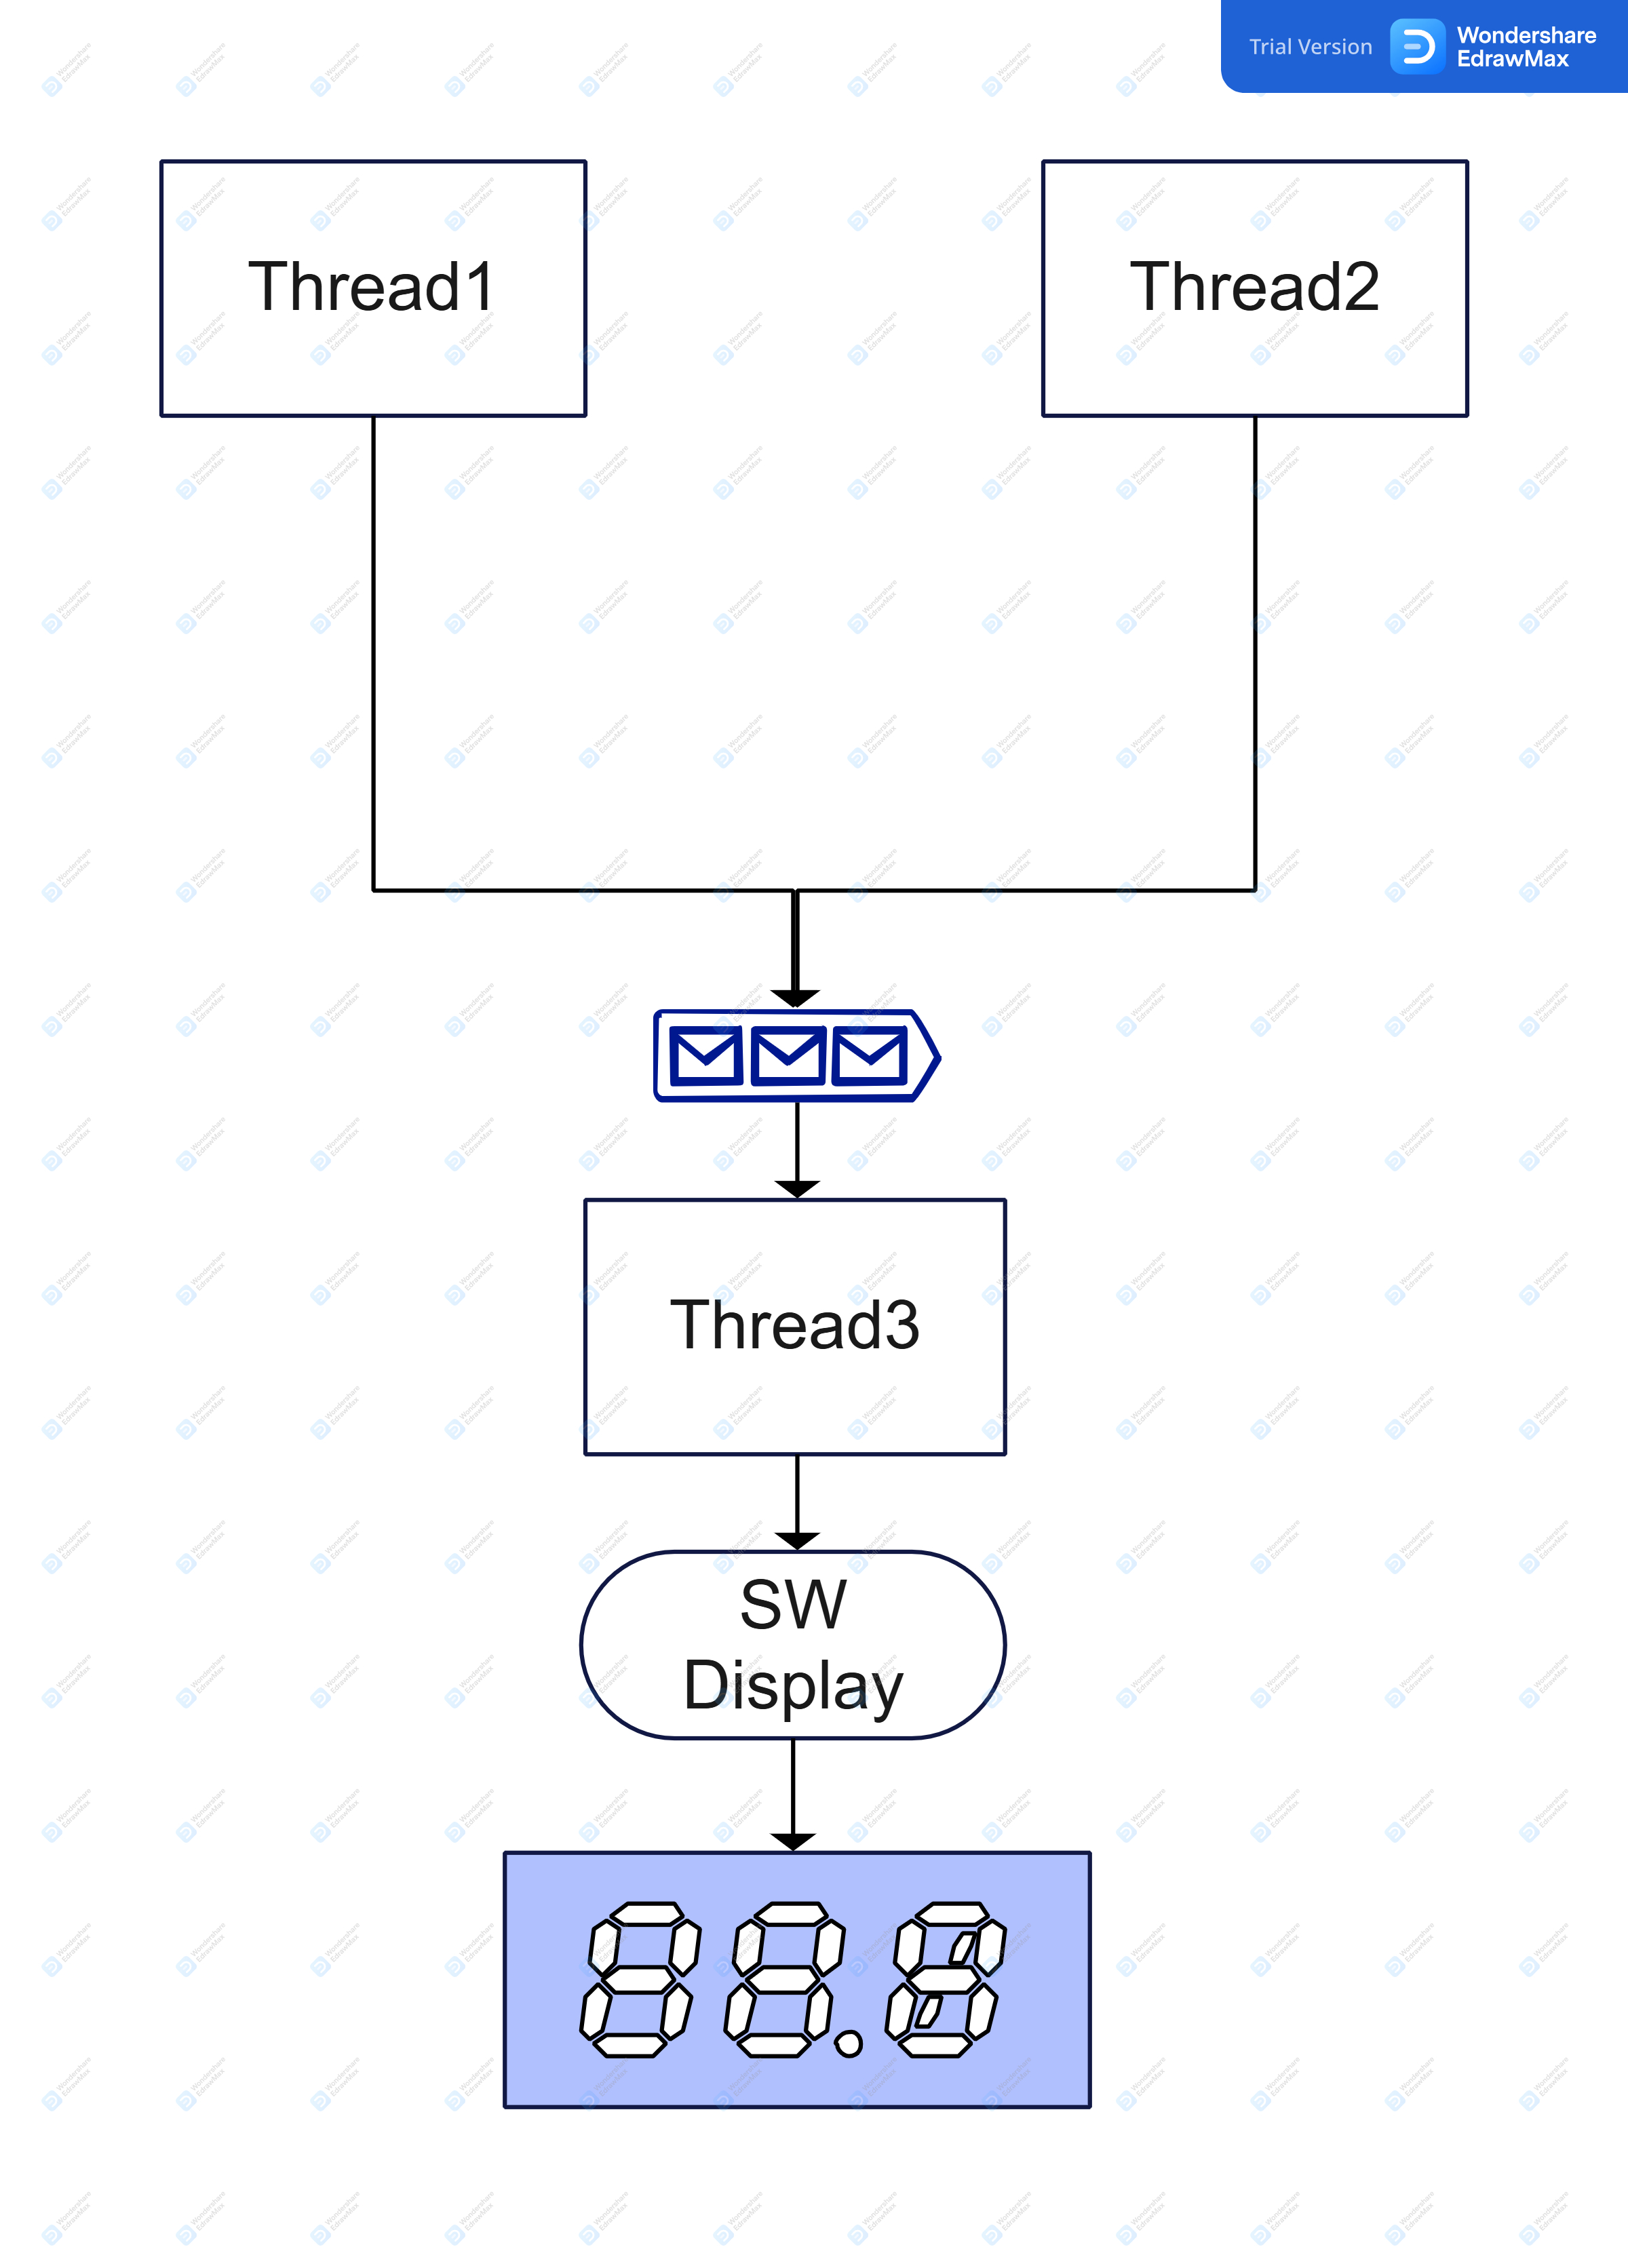
\includegraphics[scale=0.05]{threads-sync.jpg}
        \end{column}
    \end{columns}
\end{frame}



% -- Thread Flags: ejemplo ------------------------------------
\begin{frame}[fragile]{Sincronización con Thread Flags}
    \begin{itemize}
        \item \textbf{Problema}: Thread~1 genera periódicamente eventos
              (1~s). Thread~2 debe procesarlos \emph{solo} cuando estén               disponibles, esperando sin consumir CPU .
    \end{itemize}
    \begin{columns}
        \begin{column}{0.48\textwidth}
            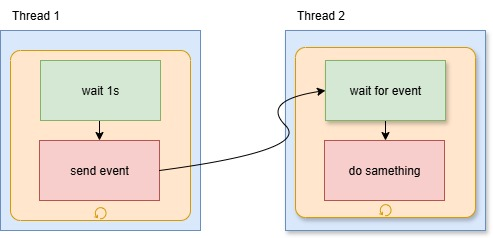
\includegraphics[scale=0.25]{flags.jpg}
            \begin{itemize}
                \item Thread~2 pasa a \textbf{Blocked} hasta que Thread~1
                      activa el flag.
                \item Al activarse, Thread~2 pasa a \textbf{Ready}.
            \end{itemize}
        \end{column}
        \begin{column}{0.52\textwidth}
            \begin{minted}[fontsize=\scriptsize, bgcolor=blue!5]{c}
void Thread1(void *arg) {
    while (1) {
        osDelay(1000);
        osThreadFlagsSet(
            tid_thread2, 0x0001U);
    }
}

void Thread2(void *arg) {
    while (1) {
        osThreadFlagsWait(  // con 's'
            0x0001U,
            osFlagsWaitAny,
            osWaitForever);
        /* procesar dato */
    }
}
            \end{minted}
        \end{column}
    \end{columns}
    \begin{alertblock}{Limitación}
        Los Thread Flags van dirigidos a \emph{un thread concreto}
        (requiere su \texttt{tid}). Para señalizar a varios threads
        simultáneamente usa \textbf{Event Flags}.
    \end{alertblock}
\end{frame}

% -- Thread Flags: API ----------------------------------------
\begin{frame}[fragile]{Thread Flags — API}
    \begin{minted}[fontsize=\scriptsize, bgcolor=blue!5]{c}
uint32_t osThreadFlagsSet(osThreadId_t thread_id, uint32_t flags)
/* Activa los flags indicados en el thread destino.
   SE PUEDE llamar desde una ISR. */

uint32_t osThreadFlagsClear(osThreadId_t thread_id, uint32_t flags)
/* Borra los flags indicados del thread activo.
   NO se puede llamar desde una ISR. */

uint32_t osThreadFlagsWait(uint32_t flags, uint32_t options,
                            uint32_t timeout)
/* Espera a que los flags estén activos.
   options: osFlagsWaitAny (cualquiera) | osFlagsWaitAll (todos).
   NO se puede llamar desde una ISR. */

uint32_t osThreadFlagsGet(void)
/* Devuelve los flags activos del thread en ejecución.
   NO se puede llamar desde una ISR. */
    \end{minted}
    \vspace{4pt}
    \href{https://arm-software.github.io/CMSIS_5/RTOS2/html/group__CMSIS__RTOS__ThreadFlagsMgmt.html}
    {CMSIS-RTOS2 Thread Flags reference}
\end{frame}

\begin{frame}

% ============================================================
%  Diagrama: Sincronización con Thread Flags (Thread1 -> Thread2)
%  + fila del Scheduler/SysTick mostrando que se ejecuta cada timeslice
%  Sustituye la imagen presentation/flags.jpg (baja calidad)
%  en el frame "Sincronización con Thread Flags"
%
%  REQUIERE en el preámbulo (si no está ya cargado):
%    \usepackage{tikz}
% ============================================================
\centering
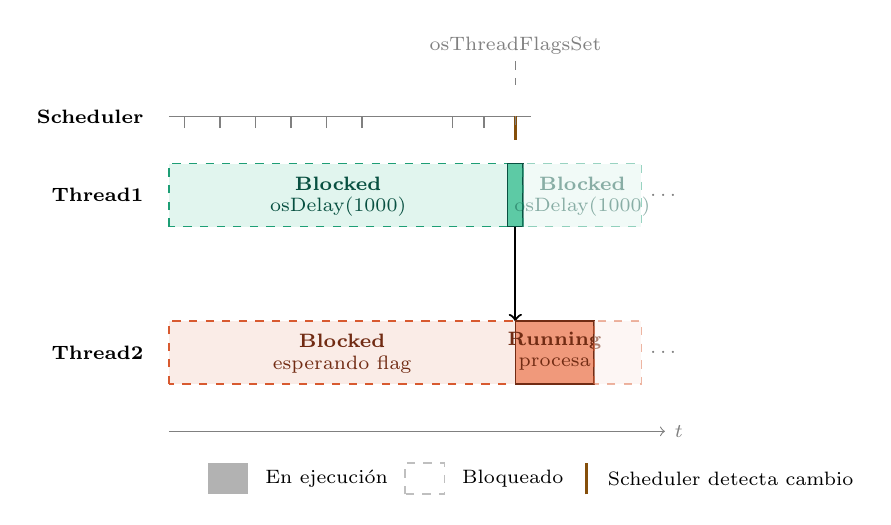
\begin{tikzpicture}[x=1cm, y=1cm, font=\scriptsize]
    % --- Colores ---
    \definecolor{tealbg}{HTML}{E1F5EE}   \definecolor{tealmid}{HTML}{5DCAA5}
    \definecolor{tealline}{HTML}{1D9E75} \definecolor{tealdark}{HTML}{085041}
    \definecolor{coralbg}{HTML}{FAECE7}  \definecolor{coralmid}{HTML}{F0997B}
    \definecolor{coralline}{HTML}{D85A30}\definecolor{coraldark}{HTML}{712B13}
    \definecolor{amberhi}{HTML}{854F0B}

    % --- Etiqueta del evento + leader hacia el tick del scheduler ---
    \node[font=\scriptsize, gray] at (4.4,3.9) {osThreadFlagsSet};
    \draw[gray, dashed, line width=0.4pt] (4.4,3.7) -- (4.4,3.4);

    % --- Fila del Scheduler / SysTick ---
    \node[anchor=east, font=\bfseries\scriptsize] at (-0.2,3.0) {Scheduler};
    \draw[gray, line width=0.5pt] (0,3.0) -- (4.6,3.0);
    \foreach \x in {0.2,0.65,1.1,1.55,2.0,2.45} {
        \draw[gray, line width=0.6pt] (\x,2.85) -- (\x,3.0);
    }
    % --- Tick resaltado: aquí el scheduler detecta el cambio ---
    \draw[amberhi, line width=1.2pt] (4.4,2.7) -- (4.4,3.0);
    \foreach \x in {3.6,4.0} {
        \draw[gray, line width=0.6pt] (\x,2.85) -- (\x,3.0);
    }

    % --- Conector corto: del tick al pulso de Thread1 ---
    \draw[gray, dashed, line width=0.4pt] (4.4,3.0) -- (4.4,2.8);

    % --- Etiquetas de los threads ---
    \node[anchor=east, font=\bfseries\scriptsize] at (-0.2,2.0) {Thread1};
    \node[anchor=east, font=\bfseries\scriptsize] at (-0.2,0.0) {Thread2};

    % --- Thread1: Blocked (osDelay) ---
    \fill[tealbg] (0,1.6) rectangle (4.3,2.4);
    \draw[tealline, dashed, line width=0.6pt] (0,1.6) rectangle (4.3,2.4);
    \node[tealdark] at (2.15,2.15) {\textbf{Blocked}};
    \node[tealdark] at (2.15,1.85) {\scriptsize osDelay(1000)};

    % --- Thread1: pulso (Running, llamada a osThreadFlagsSet) ---
    \fill[tealmid] (4.3,1.6) rectangle (4.5,2.4);
    \draw[tealdark, line width=0.6pt] (4.3,1.6) rectangle (4.5,2.4);

    % --- Thread1: continuación (siguiente ciclo, atenuado) ---
    \begin{scope}[opacity=0.45]
        \fill[tealbg] (4.5,1.6) rectangle (6.0,2.4);
        \draw[tealline, dashed, line width=0.6pt] (4.5,1.6) rectangle (6.0,2.4);
        \node[tealdark] at (5.25,2.15) {\textbf{Blocked}};
        \node[tealdark] at (5.25,1.85) {\scriptsize osDelay(1000)};
    \end{scope}
    \node[gray] at (6.3,2.0) {\ldots};

    % --- Flecha de señal: Thread1 -> Thread2 ---
    \draw[->, line width=0.8pt] (4.4,1.6) -- (4.4,0.4);

    % --- Thread2: Blocked (esperando flag) ---
    \fill[coralbg] (0,-0.4) rectangle (4.4,0.4);
    \draw[coralline, dashed, line width=0.6pt] (0,-0.4) rectangle (4.4,0.4);
    \node[coraldark] at (2.2,0.15) {\textbf{Blocked}};
    \node[coraldark] at (2.2,-0.15) {\scriptsize esperando flag};

    % --- Thread2: Running (procesa el dato) ---
    \fill[coralmid] (4.4,-0.4) rectangle (5.4,0.4);
    \draw[coraldark, line width=0.6pt] (4.4,-0.4) rectangle (5.4,0.4);
    \node[coraldark] at (4.9,0.15) {\textbf{Running}};
    \node[coraldark] at (4.9,-0.15) {\scriptsize procesa};

    % --- Thread2: continuación (atenuado, sin texto) ---
    \begin{scope}[opacity=0.45]
        \fill[coralbg] (5.4,-0.4) rectangle (6.0,0.4);
        \draw[coralline, dashed, line width=0.6pt] (5.4,-0.4) rectangle (6.0,0.4);
    \end{scope}
    \node[gray] at (6.3,0.0) {\ldots};

    % --- Eje de tiempo ---
    \draw[->, gray] (0,-1.0) -- (6.3,-1.0) node[right] {$t$};

    % --- Leyenda ---
    \fill[gray!60] (0.5,-1.8) rectangle (1.0,-1.4);
    \node[anchor=west, font=\scriptsize] at (1.1,-1.6) {En ejecución};
    \draw[gray!50, dashed, line width=0.6pt] (3.0,-1.8) rectangle (3.5,-1.4);
    \node[anchor=west, font=\scriptsize] at (3.6,-1.6) {Bloqueado};
    \draw[amberhi, line width=1.2pt] (5.3,-1.8) -- (5.3,-1.4);
    \node[anchor=west, font=\scriptsize] at (5.45,-1.6) {Scheduler detecta cambio};
\end{tikzpicture}
\end{frame}


% -- Colas: ejemplo -------------------------------------------
\begin{frame}[fragile]{CMSIS-RTOS: Colas (Message Queue)}
    \begin{itemize}
        \item Patrón \textbf{Productor/Consumidor}: un thread (o ISR)               produce datos y otro los consume de forma segura.
        \item La cola almacena \textbf{copias} del mensaje, no punteros.
    \end{itemize}
    \begin{columns}
        \begin{column}{0.48\textwidth}
            \begin{minted}[fontsize=\tiny, bgcolor=blue!5]{c}
static osMessageQueueId_t q_datos;

int Init_Threads(void) {
  q_datos = osMessageQueueNew(
                16, sizeof(uint8_t), NULL);
  osThreadNew(Producer, NULL, NULL);
  osThreadNew(Consumer, NULL, NULL);
  return 0;
}
void Producer(void *arg) {
    uint8_t idx = 0;
    while (1) {
        osMessageQueuePut(
            q_datos, &idx, 0U, 10U);
        idx++;
        osDelay(100);
    }
}
void Consumer(void *arg) {
    uint8_t val;
    while (1) {
        osMessageQueueGet(
            q_datos, &val,
            NULL, osWaitForever);  // correcto
        /* procesar val */
    }
}
            \end{minted}
        \end{column}
        \begin{column}{0.50\textwidth}
            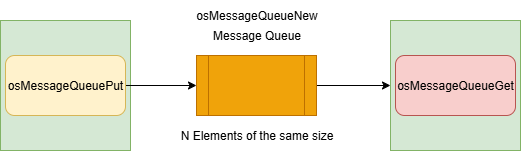
\includegraphics[scale=0.35]{queues.drawio.png}
            \begin{itemize}
                \item Si la cola está \textbf{llena}, \texttt{Put}
                      bloquea el productor (o retorna error si
                      \texttt{timeout=0}).
                \item Si la cola está \textbf{vacía}, \texttt{Get}
                      bloquea el consumidor.
            \end{itemize}
        \end{column}
    \end{columns}
\end{frame}

% -- Colas: API -----------------------------------------------
\begin{frame}[fragile]{Colas — API principal}
    \begin{minted}[fontsize=\scriptsize, bgcolor=blue!5]{c}
osMessageQueueId_t osMessageQueueNew(uint32_t msg_count,
                    uint32_t msg_size, const osMessageQueueAttr_t *attr)
/* Crea la cola: msg_count mensajes de msg_size bytes cada uno. */

osStatus_t osMessageQueuePut(osMessageQueueId_t mq_id,
                    const void *msg_ptr, uint8_t msg_prio,
                    uint32_t timeout)
/* Inserta un mensaje. Bloquea si la cola está llena y timeout > 0.
   SE PUEDE llamar desde ISR con timeout = 0. */

osStatus_t osMessageQueueGet(osMessageQueueId_t mq_id,
                    void *msg_ptr, uint8_t *msg_prio, uint32_t timeout)
/* Extrae un mensaje. Bloquea si la cola está vacía y timeout > 0.
   SE PUEDE llamar desde ISR con timeout = 0. */

uint32_t   osMessageQueueGetCount(osMessageQueueId_t mq_id)
/* Número de mensajes actualmente en la cola. */

osStatus_t osMessageQueueReset(osMessageQueueId_t mq_id)
/* Vacía la cola. */

osStatus_t osMessageQueueDelete(osMessageQueueId_t mq_id)
/* Elimina la cola y libera recursos. */
    \end{minted}
    \vspace{4pt}
    \href{https://arm-software.github.io/CMSIS_5/RTOS2/html/group__CMSIS__RTOS__Message.html}
    {CMSIS-RTOS2 Message Queue reference}
\end{frame}

% -- Timers software: concepto --------------------------------
\begin{frame}[fragile]{Timers Software — concepto}
    \begin{columns}
        \begin{column}{0.55\textwidth}
            \begin{itemize}
                \item Ejecutan una función \textbf{callback} cuando expira
                      el tiempo. No consumen un timer hardware.
                \item Dos modos:
                    \begin{itemize}
                        \item \textbf{one-shot} (\texttt{osTimerOnce}):
                              ejecuta la callback una sola vez.
                        \item \textbf{periodic} (\texttt{osTimerPeriodic}):
                              ejecuta la callback cada periodo.
                    \end{itemize}
                \item El callback se ejecuta en el contexto del
                      \textbf{osRtxTimerThread}.
                \item No configurar con periodo inferior a 1\,ms.
            \end{itemize}
            \begin{alertblock}{Restricción crítica}
                Dentro del callback \textbf{no llamar} a
                \texttt{osDelay}, \texttt{osMutexAcquire} ni ninguna
                función bloqueante. El Timer Thread es compartido por
                todos los timers.
            \end{alertblock}
        \end{column}
        \begin{column}{0.42\textwidth}
            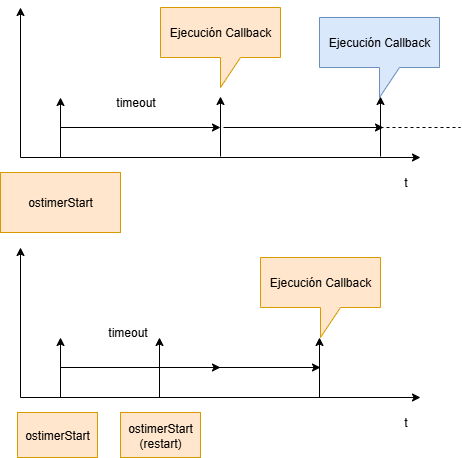
\includegraphics[scale=0.25]{softwaretimers.drawio.png}
        \end{column}
    \end{columns}
\end{frame}

% -- Timers software: ejemplo ---------------------------------
\begin{frame}[fragile]{Timers Software — ejemplo}
    \begin{columns}
        \begin{column}{0.65\textwidth}
            \begin{minted}[fontsize=\scriptsize, bgcolor=blue!5]{c}
osTimerId_t swtim_id;

/* Callback — contexto del Timer Thread
   NO llamar funciones bloqueantes aquí */
void TimerLed_Callback(void *arg) {
    LED_Toggle(LED1);
}

int Init_SWTimer(void) {
    osStatus_t status;
    Init_LED(LED1);

    swtim_id = osTimerNew(
        TimerLed_Callback,
        osTimerPeriodic,   // o osTimerOnce
        NULL, NULL);

    if (swtim_id != NULL) {
        status = osTimerStart(swtim_id, 1000U);
        if (status != osOk) { return -1; }
    }
    return 0;
}
            \end{minted}
        \end{column}
        \begin{column}{0.33\textwidth}
            \begin{itemize}
                \item \texttt{osTimerNew} crea el timer.
                \item \texttt{osTimerStart} lo arranca con
                      el periodo en ticks.
                \item Puede reiniciarse con otro
                      \texttt{osTimerStart}.
                \item \texttt{osTimerStop} lo detiene
                      sin eliminarlo.
            \end{itemize}
        \end{column}
    \end{columns}
\end{frame}

% -- Timers software: API -------------------------------------
\begin{frame}[fragile]{Timers Software — API}
    \begin{itemize}
        \item \alert{Ninguna de estas funciones se puede llamar
              desde una ISR.}
    \end{itemize}
    \begin{minted}[fontsize=\scriptsize, bgcolor=blue!5]{c}
osTimerId_t osTimerNew(osTimerFunc_t func, osTimerType_t type,
                        void *argument, const osTimerAttr_t *attr)
/* Crea el timer. type: osTimerOnce | osTimerPeriodic. */

osStatus_t osTimerStart(osTimerId_t timer_id, uint32_t ticks)
/* Arranca o reinicia el timer con el periodo indicado en ticks. */

osStatus_t osTimerStop(osTimerId_t timer_id)
/* Detiene el timer sin eliminarlo. */

uint32_t osTimerIsRunning(osTimerId_t timer_id)
/* Devuelve 1 si el timer está activo, 0 si no. */

osStatus_t osTimerDelete(osTimerId_t timer_id)
/* Elimina el timer y libera recursos. */
    \end{minted}
    \vspace{4pt}
    \href{https://arm-software.github.io/CMSIS_5/RTOS2/html/group__CMSIS__RTOS__TimerMgmt.html}
    {CMSIS-RTOS2 Timer reference}
\end{frame}

% ============================================================
\section[Configuración]{Configuración y herramientas}
% ============================================================

\begin{frame}{Estructura de un proyecto con CMSIS-RTOS}
    \resizebox{0.9\textwidth}{!}{
    \begin{forest}
    for tree={
        grow'=south, draw, rectangle,
        node options={align=center, font=\Huge\ttfamily, inner sep=14pt},
        edge path={
            \noexpand\path [draw, \forestoption{edge}]
            (!u.parent anchor) -- (.child anchor)\forestoption{edge label};
        },
    }
    [Proyecto
        [Source Group 1
            [main.c] [ThDisplay.c] [ThSensor.c] [More files]
        ]
        [\textcolor{red}{CMSIS}
            [rtx\_lib.c] [RTX\_Config.c]
            [\textcolor{green}{RTX\_Config.h}] [More files]
        ]
        [Device
            [stm32f4xx\_hal.c] [More files]
        ]
    ]
    \end{forest}}
    \begin{itemize}
        \item La figura muestra solo algunos ficheros.
        \item \textcolor{green}{\texttt{RTX\_Config.h}}: configura los
              parámetros globales del kernel.
        \item Cada periférico $\rightarrow$ un módulo
              \texttt{ThX.c}/\texttt{ThX.h} propio.
    \end{itemize}
\end{frame}

\begin{frame}{CMSIS-RTOS: Configuración de parámetros}
    \begin{table}[H]
    \centering
    \begin{tabular}{|l|l|}
    \hline
    \multicolumn{2}{|c|}{\textbf{Configuración del Sistema}} \\
    \hline
    \texttt{Global Dynamic Memory Size}    & Tamaño de la memoria dinámica \\
    \texttt{Kernel Tick Frequency}         & Frecuencia del tick (Hz) \\
    \texttt{Round-Robin Thread Switching}  & Activar Round-Robin \\
    \texttt{Round-Robin Timeout}           & Tiempo de cambio de hilo (ticks) \\
    \texttt{ISR FIFO Queue}                & Tamaño de cola FIFO para ISR \\
    \hline
    \multicolumn{2}{|c|}{\textbf{Configuración de Hilos}} \\
    \hline
    \texttt{Default Thread Stack Size}     & Pila por defecto de cada hilo \\
    \texttt{Idle Thread Stack Size}        & Pila del hilo idle \\
    \hline
    \multicolumn{2}{|c|}{\textbf{Timers Software}} \\
    \hline
    \texttt{Timer Thread Priority}         & Prioridad del Timer Thread \\
    \texttt{Timer Thread Stack Size}       & Pila del Timer Thread \\
    \hline
    \end{tabular}
    \caption{Parámetros principales de \texttt{RTX\_Config.h}}
    \end{table}
\end{frame}

\begin{frame}{Watch Window RTX — Depuración del RTOS}
    \begin{columns}
        \begin{column}{0.52\textwidth}
            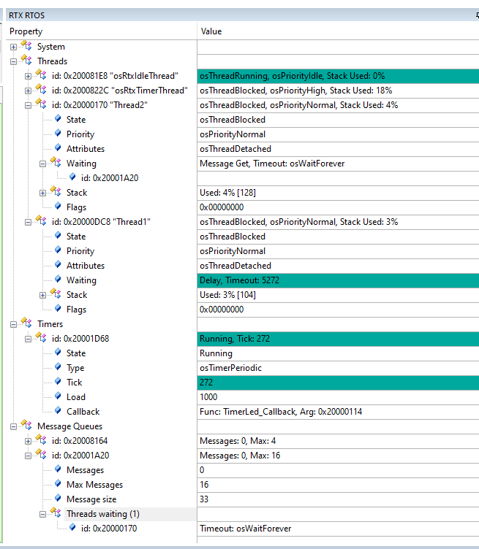
\includegraphics[width=\textwidth]{watchwindowRTX.png}
        \end{column}
        \begin{column}{0.46\textwidth}
            \begin{itemize}
                \item \textbf{osRtxIdleThread}: thread idle del SO.
                \item \textbf{osRtxTimerThread}: gestiona los timers
                      software.
                \item \textbf{Thread1, Thread2\ldots}: threads de la
                      aplicación — estado, prioridad y uso de pila.
                \item \textbf{Timers}: tipo, periodo y estado de cada
                      timer.
                \item \textbf{Message Queues}: mensajes en cola,
                      capacidad y threads bloqueados.
            \end{itemize}
            \vspace{4pt}
            {\footnotesize Keil MDK: \emph{View} $\rightarrow$
             \emph{Watch Windows} $\rightarrow$ \emph{RTX RTOS}.}
        \end{column}
    \end{columns}
\end{frame}

% ============================================================
\section[Consideraciones]{Consideraciones finales}
% ============================================================

\begin{frame}{CMSIS-RTOS: Consideraciones de diseño para SBM}
    \begin{itemize}
        \item Diseñar la estructura antes de codificar. Prestar especial atención a la sincronización entre threads.
        \item Cada periférico está gestionado por un módulo con su thread, señales, colas y estructuras de datos. Todas las operaciones con el periférico se gestionan a través de su cola.
        \item Las ISRs serán cortas: la HAL llama a las callbacks; desde ellas solo se activa flag o se envia mensaje a cola, nunca bucles ni funciones bloqueantes. Verificar qué funciones del SO se pueden usar en una ISR.
        \item Reducir al mínimo el uso de variables globales: pasar datos mediante colas o semáforos.
    \end{itemize}
\end{frame}

\begin{frame}{Buenas prácticas}
    \begin{itemize}
        \item \textbf{Dimensionar la pila correctamente}: usar la Watch Window para comprobar el uso real. Un desbordamiento de pila  produce comportamiento impredecible.
        \item \textbf{No bloquear en callbacks de timer}: el \texttt{osRtxTimerThread} es compartido por todos los timers; bloquearlo afecta a todos ellos.
        \item \textbf{Cuidado con las prioridades}: Mantener todos los threads con la misma prioridad salvo causa justificada. Un thread de alta prioridad que nunca se bloquea impide la ejecución del resto. 
        \item En SBM no se van a utilizar Event Flags, ni\textbf{Mutex}, ni \textbf{semáforo}. En caso muy justificados puede ser necesario. Están explicados en la parte Avanzada
        \item Optativo: \textbf{Nombrar los objetos del SO} con \texttt{osThreadAttr\_t},             \texttt{osMutexAttr\_t}\ldots: aparecen en la Watch Window y facilitan la depuración.
    \end{itemize}
\end{frame}

% -- Tabla resumen --------------------------------------------
\begin{frame}{¿Qué mecanismo de sincronización usar?}
    \scriptsize
    \begin{table}[H]
    \centering
    \begin{tabular}{|p{3.2cm}|p{4.5cm}|p{3.2cm}|}
    \hline
    \textbf{Mecanismo} & \textbf{Cuándo usarlo} & \textbf{Desde ISR} \\
    \hline
    \textbf{Thread Flags}
        & Señal a un thread concreto (se conoce el \texttt{identificador})
        & Sí (\texttt{osThreadFlagsSet}) \\
    \hline
    \textbf{Cola}
        & Paso de datos entre threads o ISR~$\to$~thread
        & Sí (\texttt{osMessageQueuePut }, \texttt{timeout=0}) \\
    \hline
    \textbf{Event Flags}
        & Señal broadcast a varios threads
        & Sí (\texttt{Set}) \\
    \hline
    \textbf{Mutex}
        & Proteger recurso compartido (threads únicamente)
        & No \\
    \hline
    \textbf{Semáforo binario}
        & Señalización ISR~$\to$~thread; fin de operación HW
        & Sí (\texttt{Release}) \\
    \hline
    \textbf{Semáforo contador}
        & Pool de N recursos; conteo de eventos
        & Sí (\texttt{Release}) \\
    \hline
    \end{tabular}
    \end{table}
    \begin{exampleblock}{Importante}
         En la asignatura no vamos a usar Event Flags, ni Mutex ni los semáforos porque vamos a simplificar la sincronización usando Colas y Thread Flags fundamentalmente
     \end{exampleblock}
\end{frame}

\begin{frame}{Ejercicios — Repositorio de ejemplos}
    \begin{itemize}
        \item Código en GitHub:
              \href{https://github.com/mruizglz/SBM-rtos}{mruizglz/SBM-rtos}
        \item Documentación:
              \href{https://mruizglz.github.io/SBM-rtos}{Sphinx HTML} |
              \href{https://mruizglz.github.io/SBM-rtos/simplepdf/SBM-CMSIS-RTOS-V2.pdf}{PDF}
        \item Ejemplos disponibles:
            \begin{itemize}
                \item \texttt{threads} — Creación de dos threads usando la
                      misma función
                \item \texttt{threads-flags} — Sincronización con Thread Flags
                \item \texttt{threads-queues} — Sincronización con colas
                \item \texttt{threads-timers} — Uso de timers virtuales
            \end{itemize}
        \item \textbf{Próximamente}: \texttt{threads-mutex},
              \texttt{threads-semaphore}
    \end{itemize}
\end{frame}

\section[Avanzado]{Uso avanzado de la sincronización}
% -- Mutex: concepto ------------------------------------------
\begin{frame}[fragile]{Mutex — Exclusión Mutua}
    \begin{itemize}
        \item Un \textbf{mutex} garantiza que solo \emph{un} thread a la
              vez accede a un recurso compartido.
        \item El thread que lo adquiere es el \textbf{propietario único};
              debe liberarlo cuando termine de usar el recurso.
        \item RTX5 soporta \textbf{priority inheritance}: eleva
              temporalmente la prioridad del propietario para evitar
              inversión de prioridad.
    \end{itemize}
    \begin{minted}[fontsize=\scriptsize, bgcolor=blue!5]{c}
osMutexId_t mutex_display;

// Crear en la inicialización
mutex_display = osMutexNew(NULL);

// Thread A
osMutexAcquire(mutex_display, osWaitForever); // bloquea si ocupado
    /* --- sección crítica: acceso exclusivo al recurso --- */
osMutexRelease(mutex_display);

// Thread B — espera hasta que A libere
osMutexAcquire(mutex_display, osWaitForever);
    /* --- sección crítica --- */
osMutexRelease(mutex_display);
    \end{minted}
    \scriptsize
    \begin{alertblock}{Regla}
        El mismo thread que adquiere el mutex \textbf{debe} liberarlo.
        \texttt{osMutexAcquire/Release} \textbf{no se pueden llamar
        desde una ISR}.
    \end{alertblock}
\end{frame}

% -- Mutex: API -----------------------------------------------
\begin{frame}[fragile]{Mutex — API}
    \begin{minted}[fontsize=\scriptsize, bgcolor=blue!5]{c}
osMutexId_t osMutexNew(const osMutexAttr_t *attr)
/* Crea e inicializa un mutex. Devuelve NULL si falla.
   Para activar priority inheritance:
       const osMutexAttr_t attr = {.attr_bits = osMutexPrioInherit};  */

osStatus_t osMutexAcquire(osMutexId_t mutex_id, uint32_t timeout)
/* Adquiere el mutex. Bloquea el thread si está ocupado.
   timeout = osWaitForever → espera indefinida.
   NO se puede llamar desde una ISR. */

osStatus_t osMutexRelease(osMutexId_t mutex_id)
/* Libera el mutex. Debe llamarlo el mismo thread que lo adquirió.
   NO se puede llamar desde una ISR. */

osMutexId_t osMutexGetOwner(osMutexId_t mutex_id)
/* Devuelve el thread que actualmente posee el mutex. */

osStatus_t osMutexDelete(osMutexId_t mutex_id)
/* Elimina el mutex y libera sus recursos. */
    \end{minted}
    \vspace{4pt}
    \href{https://arm-software.github.io/CMSIS_5/RTOS2/html/group__CMSIS__RTOS__MutexMgmt.html}
    {CMSIS-RTOS2 Mutex reference}
\end{frame}


% -- Semáforo: concepto ---------------------------------------
\begin{frame}[fragile]{Semáforo — Señalización y Conteo}
    \begin{itemize}
        \item Un \textbf{semáforo} tiene un contador interno.
              \texttt{Release} incrementa; \texttt{Acquire} decrementa
              (o bloquea si el contador es~0).
        \item A diferencia del mutex, \textbf{cualquier thread o ISR}
              puede hacer \texttt{Release} — no hay propietario.
        \item Usos principales:
            \begin{itemize}
                \item \textbf{Binario} (inicial=0): señalizar desde una
                      ISR/callback a un thread que espera.
                \item \textbf{Contador} (inicial=N): controlar el acceso
                      a un pool de N recursos.
            \end{itemize}
    \end{itemize}
    \begin{minted}[fontsize=\scriptsize, bgcolor=blue!5]{c}
// Semáforo binario: señalización ISR → thread
osSemaphoreId_t sem_dato;
sem_dato = osSemaphoreNew(1, 0, NULL); // máx=1, inicial=0

// Desde la ISR o callback (se puede llamar desde interrupción):
osSemaphoreRelease(sem_dato);          // "hay un dato listo"

// En el thread — se bloquea hasta que la ISR libere:
osSemaphoreAcquire(sem_dato, osWaitForever);
/* procesar el dato */
    \end{minted}
    \begin{alertblock}{Mutex vs Semáforo}
        Usa \textbf{mutex} para exclusión mutua (mismo thread adquiere
        y libera). Usa \textbf{semáforo} para señalización (uno produce,
        otro consume).
    \end{alertblock}
\end{frame}

% -- Semáforo: API --------------------------------------------
\begin{frame}[fragile]{Semáforo — API}
    \begin{minted}[fontsize=\scriptsize, bgcolor=blue!5]{c}
osSemaphoreId_t osSemaphoreNew(uint32_t max_count,
                               uint32_t initial_count,
                               const osSemaphoreAttr_t *attr)
/* Crea un semáforo.
   Semáforo binario:   osSemaphoreNew(1, 0, NULL)  → señalización
   Semáforo contador:  osSemaphoreNew(3, 3, NULL)  → pool de 3 recursos */

osStatus_t osSemaphoreAcquire(osSemaphoreId_t semaphore_id,
                               uint32_t timeout)
/* Decrementa el contador. Bloquea si contador == 0.
   Desde ISR: SOLO si timeout == 0. */

osStatus_t osSemaphoreRelease(osSemaphoreId_t semaphore_id)
/* Incrementa el contador. Despierta un thread bloqueado si lo hay.
   SE PUEDE llamar desde una ISR. */

uint32_t osSemaphoreGetCount(osSemaphoreId_t semaphore_id)
/* Devuelve el valor actual del contador. */

osStatus_t osSemaphoreDelete(osSemaphoreId_t semaphore_id)
/* Elimina el semáforo y libera recursos. */
    \end{minted}
    \vspace{4pt}
    \href{https://arm-software.github.io/CMSIS_5/RTOS2/html/group__CMSIS__RTOS__SemaphoreMgmt.html}
    {CMSIS-RTOS2 Semaphore reference}
\end{frame}

% -- Event Flags ----------------------------------------------
\begin{frame}[fragile]{Event Flags — Señalización a múltiples threads}
    \begin{itemize}
        \item Los \textbf{Event Flags} son un objeto independiente (no
              ligado a ningún thread) que puede ser esperado por
              \emph{varios} threads a la vez.
        \item Útil cuando un evento (p.ej.\ una interrupción) debe
              despertar a varios threads simultáneamente.
    \end{itemize}
    \begin{minted}[fontsize=\scriptsize, bgcolor=blue!5]{c}
osEventFlagsId_t evt_datos;

// Crear (en la inicialización)
evt_datos = osEventFlagsNew(NULL);

// Desde cualquier thread o ISR — activa el bit 0
osEventFlagsSet(evt_datos, 0x0001U);       // SE PUEDE llamar desde ISR

// Thread A — espera bit 0
osEventFlagsWait(evt_datos, 0x0001U,
                 osFlagsWaitAny, osWaitForever);

// Thread B — también espera bit 0 (ambos se despiertan)
osEventFlagsWait(evt_datos, 0x0001U,
                 osFlagsWaitAny, osWaitForever);
    \end{minted}
    \vspace{4pt}
    \href{https://arm-software.github.io/CMSIS_5/RTOS2/html/group__CMSIS__RTOS__EventFlags.html}
    {CMSIS-RTOS2 Event Flags reference}
\end{frame}